\documentclass{beamer}

\usetheme{default}
\usecolortheme{beaver}

\usepackage[german]{babel}
\usepackage[utf8]{inputenc}

\usepackage[sfdefault]{roboto}
\usepackage{textcomp}

\usepackage{graphicx}
\graphicspath{{./images/}}

\usepackage{subfig}

\setbeamertemplate{navigation symbols}{}

\AtBeginSection[]{
  \begin{frame}
  \vfill
  \centering
  \begin{beamercolorbox}[sep=8pt,center]{title}
    \usebeamerfont{title}\insertsectionhead\par%
  \end{beamercolorbox}
  \vfill
  \end{frame}
}

\title{How To Uni @ PROLOG 2020}
\date{WS 2020/21}
\author{Lukas Anzinger}

\begin{document}

\begin{frame}
    \maketitle
\end{frame}

\begin{frame}{Was euch heute erwartet}
    \setcounter{tocdepth}{1}
    \tableofcontents
\end{frame}

\section{Die FSINF stellt sich vor}

\begin{frame}{Was ist die FSINF?}
    Die FSINF ist ...
    \begin{itemize}
        \item ... die Fachschaft Informatik
        \item ... eine (lose) Gruppe von Studierenden (darunter auch die
            \textit{gewählten} Studienvertreter\_innen)
        \item ... deine Interessensvertretung als Informatikstudent\_in!
    \end{itemize}
\end{frame}

\begin{frame}{Was macht die FSINF für euch?}
    Ansprechpartner für ...
    \begin{itemize}
        \item Fragen zum Studium
        \item Organisatorische Fragen
        \item Probleme mit LVAs oder Profs
    \end{itemize}
\end{frame}

\begin{frame}{Wo findet ihr die FSINF?}
    \begin{figure}[htp]
        \centering
        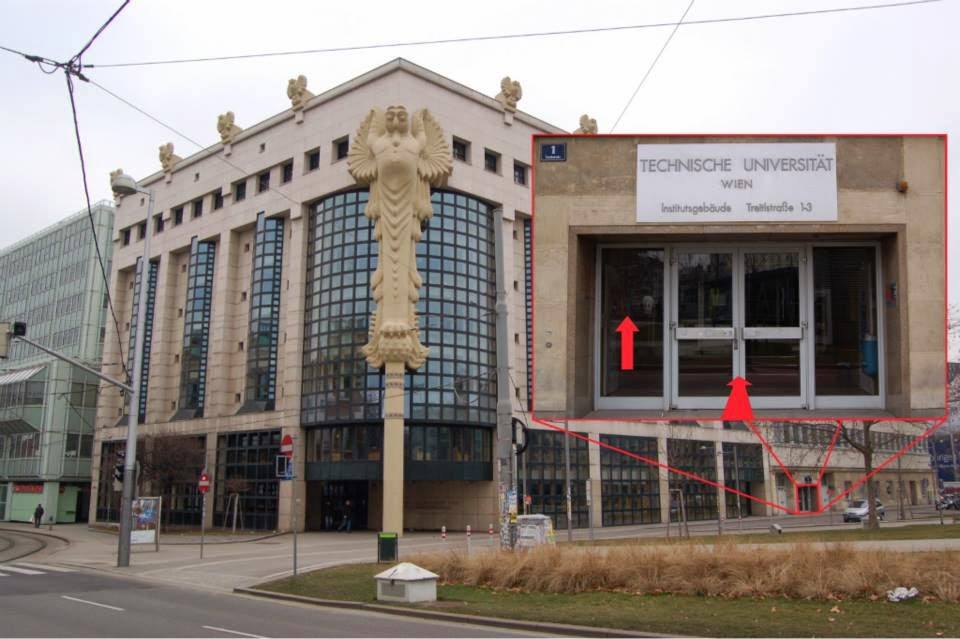
\includegraphics[width=\textwidth]{fsinf.jpg}
        \caption{So geht's zur FSINF: Treitlstraße 1-3, im Hochpaterre}
    \end{figure}
\end{frame}

\begin{frame}{Wo findet ihr die FSINF?}
    \begin{figure}[htp]
        \centering
        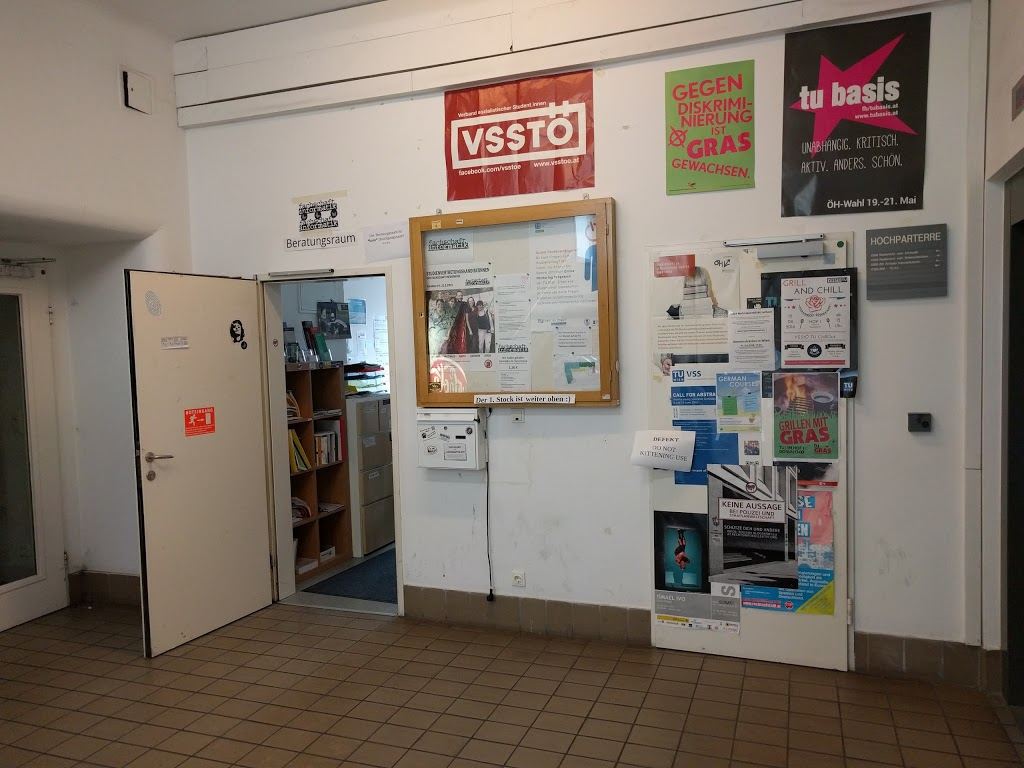
\includegraphics[width=0.8\textwidth]{eingang.jpg}
        \caption{Eingang zur FSINF (im Hochpaterre)}
    \end{figure}
\end{frame}

\begin{frame}{Was bietet euch die FSINF?}
    \begin{itemize}
        \item Beratung
        \item Räumlichkeiten (2 Lernräume + 1 Beratungsraum)
        \item Küche
        \item Ort zum Socializen
        \item Gekühlte Getränke
        \item Kaffee
    \end{itemize}
\end{frame}

\begin{frame}{Was bietet euch die FSINF?}
    \begin{figure}[htp]
        \centering
        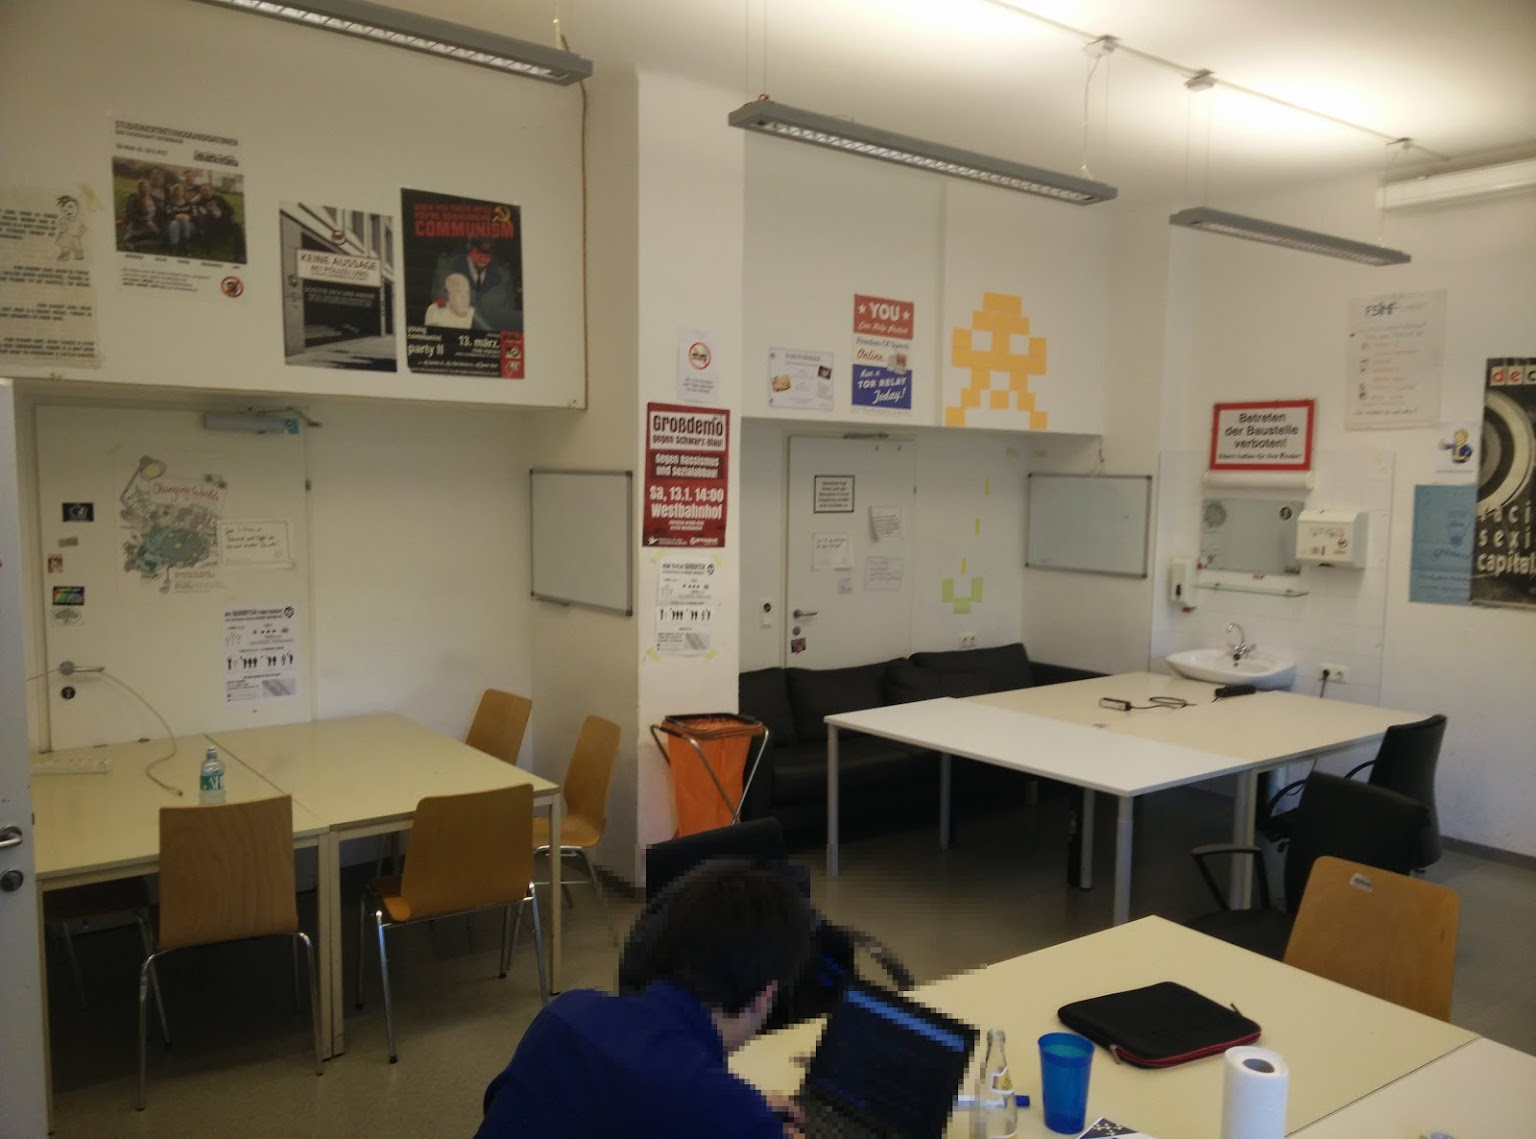
\includegraphics[width=0.9\textwidth]{lernraum.jpg}
        \caption{Lernraum 1}
    \end{figure}
\end{frame}

\begin{frame}{Was bietet euch die FSINF?}
    \begin{figure}[htp]
        \centering
        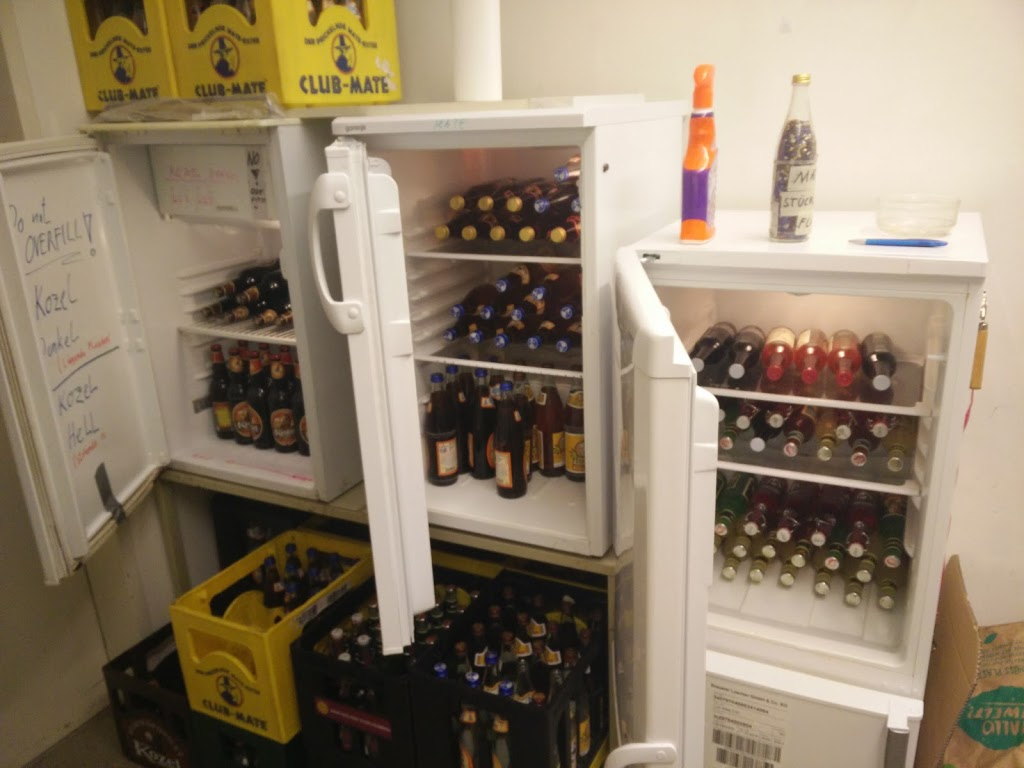
\includegraphics[width=0.9\textwidth]{kuehlschrank.jpg}
        \caption{Club Mate, Kozel und andere Getränke}
    \end{figure}
\end{frame}

\begin{frame}{Was bietet euch die FSINF?}
    \begin{figure}[htp]
        \centering
        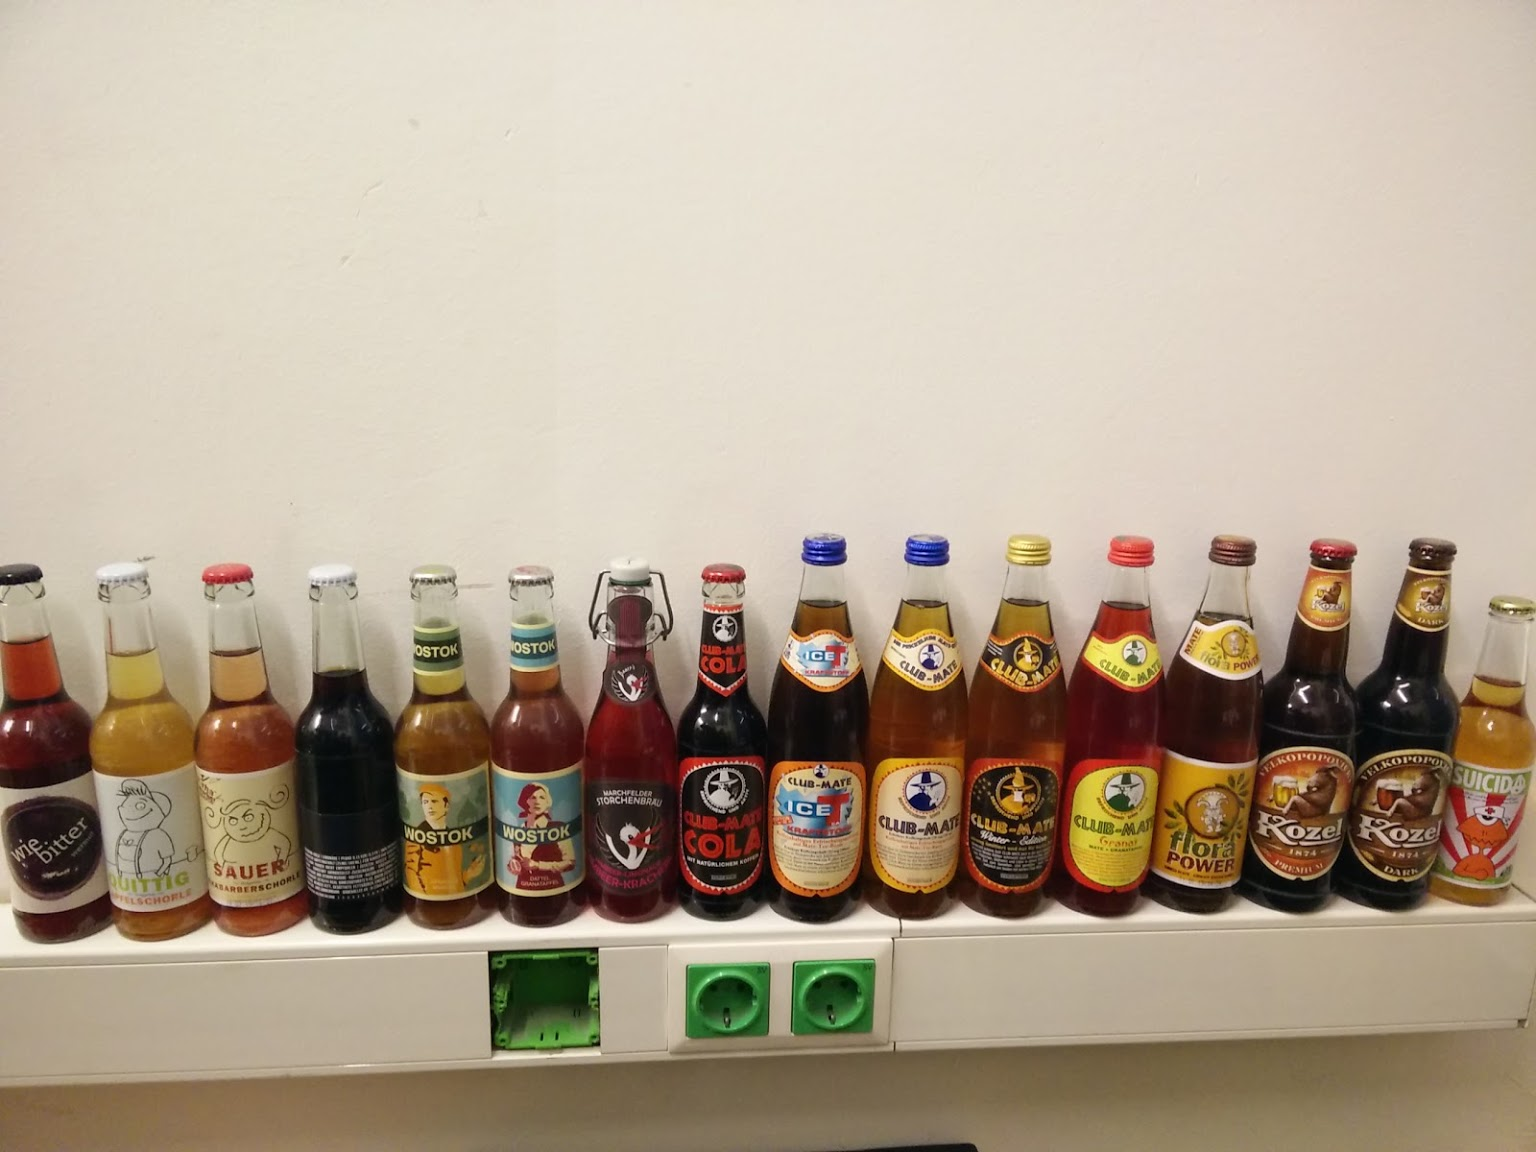
\includegraphics[width=0.9\textwidth]{getraenke.jpg}
        \caption{Eine Vielzahl von Getränken zu Studi-freundlichen Preisen}
    \end{figure}
\end{frame}

\begin{frame}{Wie erreicht ihr die FSINF?}
    \begin{itemize}
        \item Mattermost (Chat): https://mm.fsinf.at
        \item Homepage: https://www.fsinf.at
        \item Telefon: +43 1 58801 49550
        \item E-Mail: fsinf@fsinf.at
        \item Beratung: beratung@fsinf.at
    \end{itemize}
\end{frame}

\begin{frame}{Wann ist die FSINF offen?}
    \begin{itemize}
        \item Theoretisch: Immer offen, wenn Leute da sind
        \item Praktisch: Auf gut Glück probieren, anrufen oder im Mattermost nachfragen
        \item Lernraumschlüssel können auch ausgeborgt werden
    \end{itemize}
\end{frame}

\begin{frame}{Wie arbeiten wir?}
    \begin{itemize}
        \item nicht-hierarchisch
        \item in unserer Freizeit
        \item unbezahlt
        \item freiwillig
        \item unfraktioniert, aber politisch
        \item nicht nur während des Semesters
    \end{itemize}
\end{frame}

\begin{frame}{Digitale Services}
    \begin{itemize}
        \item VoWi (Wiki): https://vowi.fsinf.at
        \item Mattermost (Chat): https://mm.fsinf.at
        \item TOSS (Suche): https://toss.fsinf.at
    \end{itemize}
\end{frame}

\begin{frame}{VoWi}
  \begin{columns}
    \column{0.60\linewidth}
      \centering
      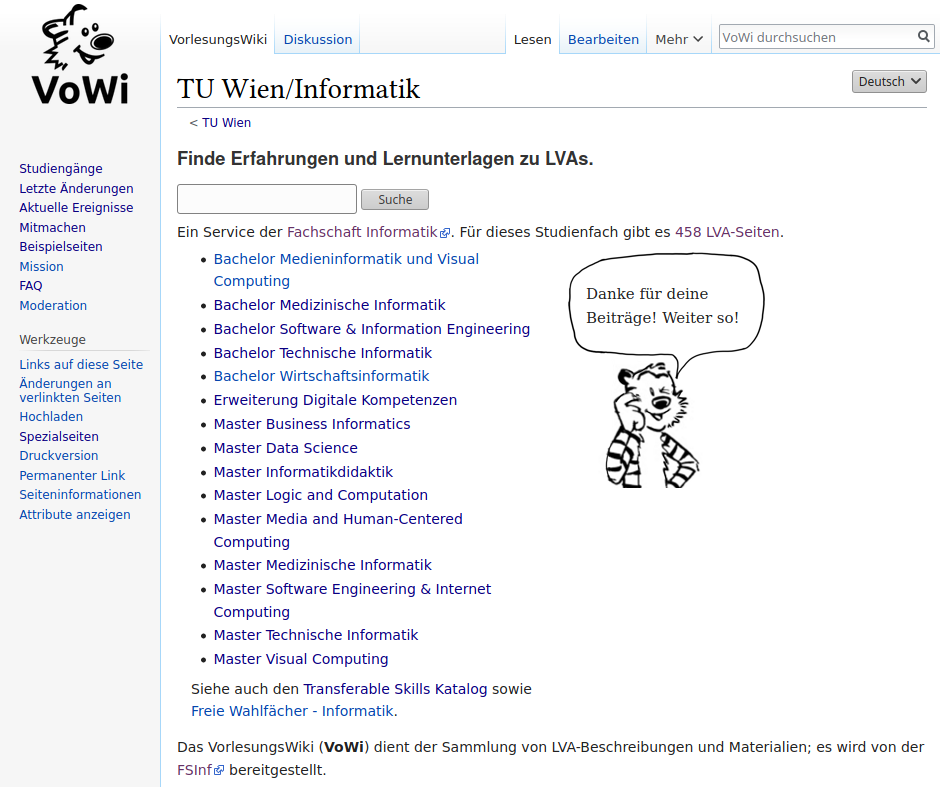
\includegraphics[width=\textwidth]{vowi.png}
      https://vowi.fsinf.at
    \column{0.50\linewidth}
      \begin{itemize}
        \item Wiki zu Lehrveranstaltungen
        \item Wichtige Quelle für Materialien
        \item Sammlung von gelösten Übungen, alten Prüfungen, Zusammenfassungen,
            Erfahrungsberichte
        \item Sei mutig und trage bei!
      \end{itemize}
  \end{columns}
\end{frame}

\begin{frame}{Mattermost (1)}
  \begin{columns}
    \column{0.60\linewidth}
      \centering
      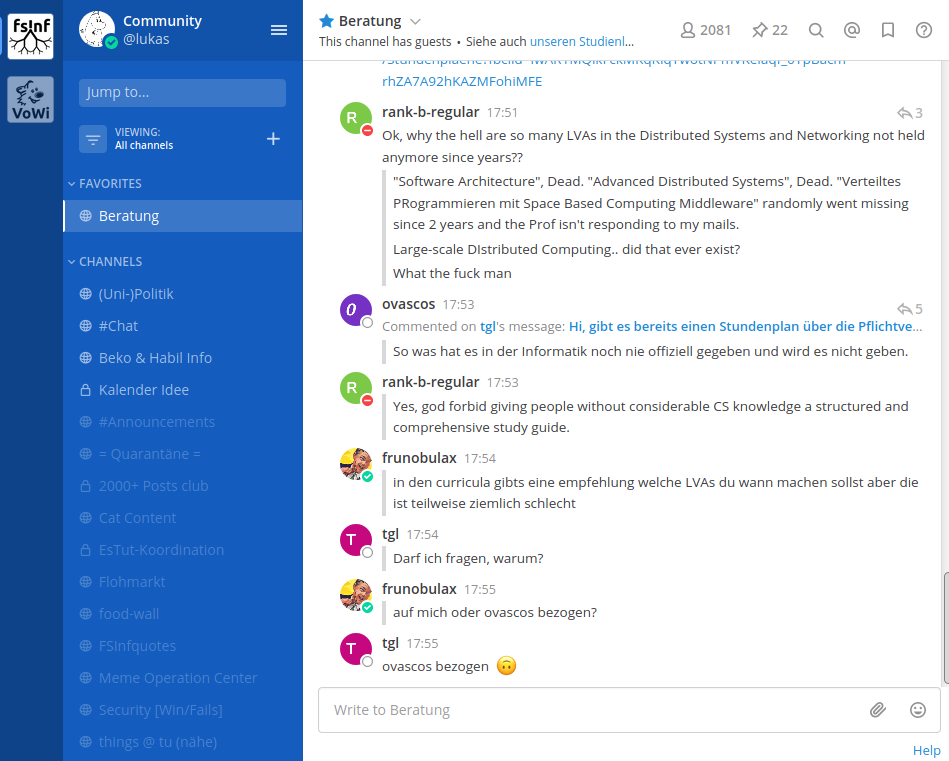
\includegraphics[width=\textwidth]{mattermost.png}
      https://mm.fsinf.at
    \column{0.50\linewidth}
      \begin{itemize}
        \item Selbst-gehosteter Messaging Service/Chat
        \item Eure Daten sind bei uns sicher
        \item Anmeldung mit eurer Studi-Mail-Adresse
        \item Kontakt zu anderen Studis, Tutoren, FSINF-Team, ...
        \item Eigener Channel für jede LVA
      \end{itemize}
  \end{columns}
\end{frame}

\begin{frame}{Mattermost (2)}
  \begin{columns}
    \column{0.60\linewidth}
      \centering
      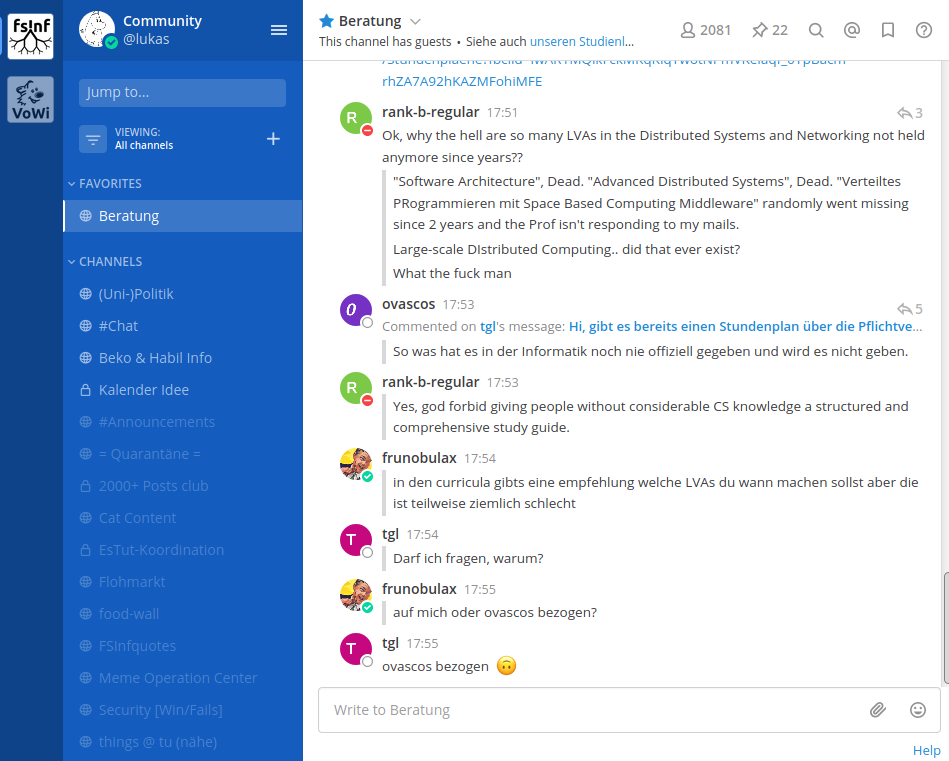
\includegraphics[width=\textwidth]{mattermost.png}
      https://mm.fsinf.at
    \column{0.50\linewidth}
      \begin{itemize}
        \item Off-Topic-Channels zum Socializen
        \item Interessante Mattermost-Channels:
            \begin{itemize}
                \item Beratung
                \item (Lern)Räume
                \item EsTuts
                \item Food-Wall
                \item Meme Operation Center
            \end{itemize}
      \end{itemize}
  \end{columns}
\end{frame}

\begin{frame}{TOSS}
  \begin{columns}
    \column{0.60\linewidth}
      \centering
      
\includegraphics[width=\textwidth]{toss.png}
      https://toss.fsinf.at
    \column{0.50\linewidth}
      \begin{itemize}
        \item Suchmaschine der FSINF
        \item Suche in Vielzahl an Quellen:
        \begin{itemize}
            \item TISS-LVAs
            \item Mattermost-Channels
            \item VoWi-Seiten
            \item Räumen
            \item uvm.
        \end{itemize}
      \end{itemize}
  \end{columns}
\end{frame}

\section{Organisatorisches}

\begin{frame}{Studieneingangs- und Orientierungsphase (STEOP)}
    \begin{itemize}
        \item Am Anfang könnt ihr nur LVAs aus den ersten 2 Semestern belegen
        \item Erst nach Erfüllung der STEOP könnt ihr alle (weiteren) LVAs
              absolvieren
        \item \textbf{Wichtig:} Algebra VO, EPROG 1 VU, Orientierung VU
              müsst ihr auf jeden Fall positiv absolvieren
        \item Außerdem müsst ihr 6 ECTS aus dem STEOP-Pool machen,
              z.\,B. Technische Grundlagen der Informatik VU
    \end{itemize}
    \begin{figure}[htp]
        \centering
        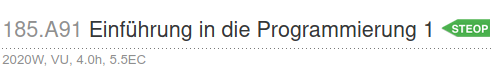
\includegraphics[width=1\textwidth]{tiss_steop_marker.png}
        \caption{STEOP-LVAs sind in TISS grün gekennzeichnet}
    \end{figure}
\end{frame}

\begin{frame}{STEOP nicht komplett geschafft, was nun?}
    \begin{itemize}
        \item Die LVAs des 1. und 2. Semesters
        \item Freie Wahlfächer und Transferable Skills
    \end{itemize}
    \ldots\ benötigen \textit{keine} STEOP!\\
\end{frame}

\section{TISS}
\begin{frame}{TISS: Wichtigste Funktionen}
    \begin{itemize}
        \item Favoriten
        \item LVA-Kataloge
        \item Studienplan
        \item Zeugnisse \& Bestätigungen
    \end{itemize}
    \vspace{2cm}
    \centering \small Mehr: https://tiss.tuwien.ac.at/hilfe/zu/tiss/new\_erste\_info\_stud
\end{frame}

\begin{frame}{TISS: Login}
    \begin{figure}[htp]
        \centering
        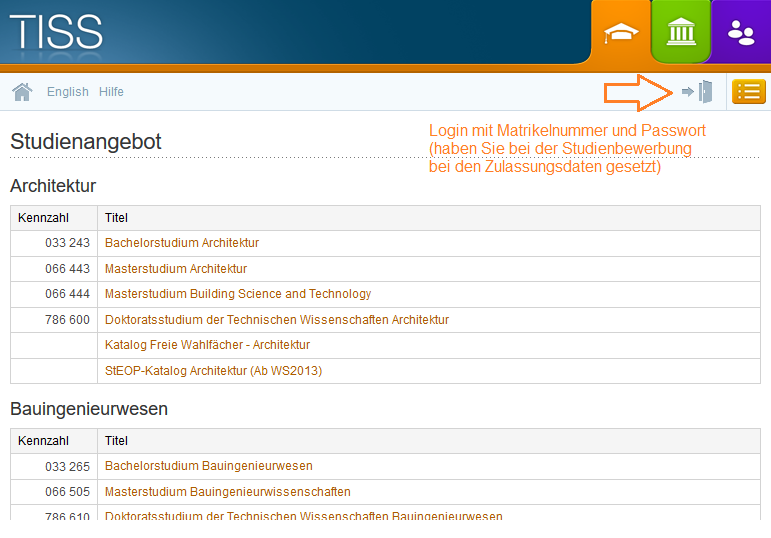
\includegraphics[width=1\textwidth]{tiss_login.png}
    \end{figure}
\end{frame}

\begin{frame}{TISS: Studienangebot}
    \begin{figure}[htp]
        \centering
        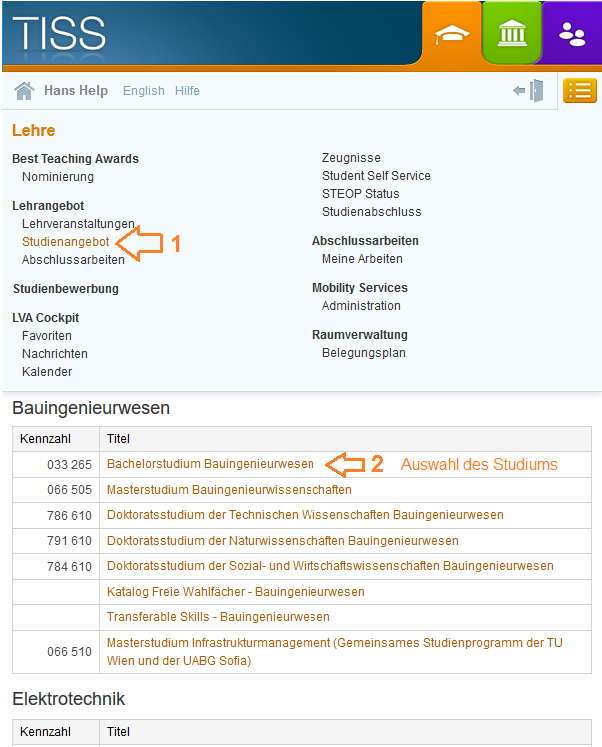
\includegraphics[width=0.9\textwidth]{tiss_studienangebot.png}
    \end{figure}
\end{frame}

\begin{frame}{TISS: LVA}
    \begin{figure}[htp]
        \centering
        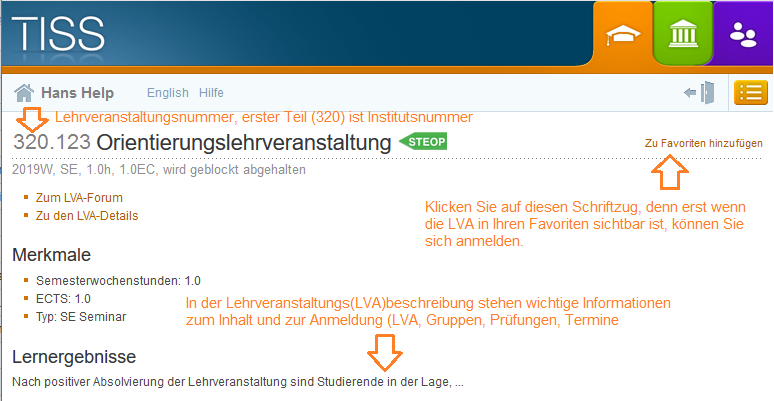
\includegraphics[width=1\textwidth]{tiss_lva.png}
    \end{figure}
\end{frame}

\begin{frame}{TISS: Favoriten}
    \begin{figure}[htp]
        \centering
        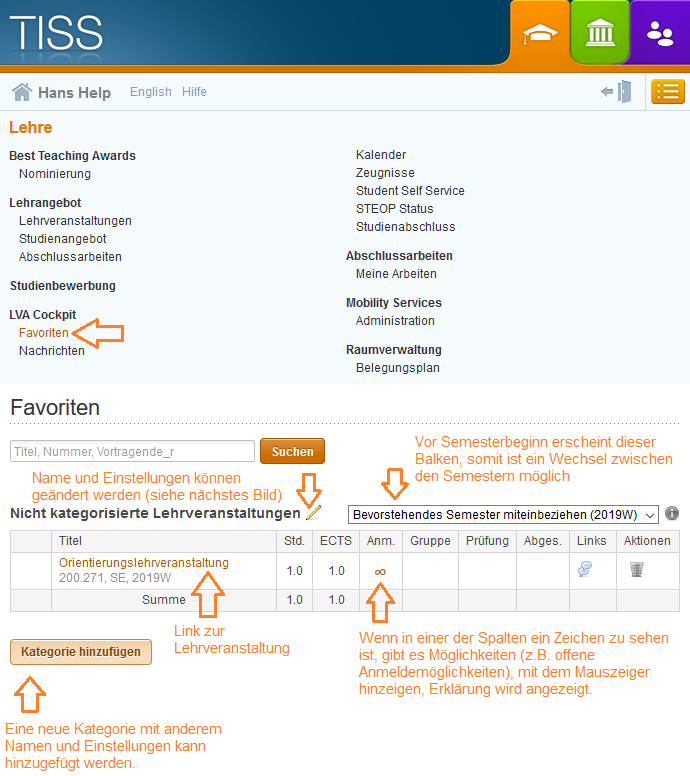
\includegraphics[width=0.6\textwidth]{tiss_favoriten.png}
    \end{figure}
    \centering \textbf{Achtung:} Ersetzt nicht die Anmeldung!
\end{frame}

\section{LVAs}

\begin{frame}{Welche LVAs soll ich machen?}
    \begin{itemize}
        \item Studienplan
        \item Semesterempfehlung im Studienplan
        \item Jedes Informatik-Studium hat eigenen Studienplan
    \end{itemize}
\end{frame}

\begin{frame}{Wo bekomme ich Infos zu einer LVA?}
    \begin{itemize}
        \item Im TISS nach LVA suchen: Termine, Leistungsnachweis, Anmeldung
        \item 1. Einheit der LVA == Vorbesprechung
        \item Im TUWEL-Kurs (nach Anmeldung im TISS)
        \item Im VoWi: https://vowi.fsinf.at
    \end{itemize}
\end{frame}

\begin{frame}{Wie melde ich mich zu einer LVA an?}
    \begin{itemize}
        \item Im TISS auf der LVA-Seite
        \item Oft: Zusätzliche Anmeldung für Prüfung und/oder Gruppe erforderlich
    \end{itemize}
\end{frame}

\section{Infrastruktur an der TU Wien}

\begin{frame}{Mail-Adresse}
    \begin{itemize}
        \item Automatisch zugeteilt: e(matrikelnummer)@student.tuwien.ac.at
        \item Zusätzlich (freiwillig registrierbar): (vorname).(nachname)@student.tuwien.ac.at
        \item \url{https://webmail.tuwien.ac.at}
        \item Weiterleitung auf private Adresse möglich
    \end{itemize}
\end{frame}

\begin{frame}{Software für Studierende}
    \begin{itemize}
        \item z.\,B. Office 365 um 3{,}65 €, Windows 10 Pro um 8 €, ...
        \item \url{http://www.sss.tuwien.ac.at/sss/}
    \end{itemize}
\end{frame}

\begin{frame}{WLAN/VPN}
    \begin{itemize}
        \item Nur TUNET + eduroam verschlüsselt
        \item VPN: \url{https://www.it.tuwien.ac.at/services/netzwerkinfrastruktur-und-serverdienste/tunet/vpn-virtual-private-network/vpn-zugang/}
    \end{itemize}
\end{frame}

\begin{frame}{Bibliothek}
    \begin{itemize}
        \item Bücher in der Hauptbücherei (Gebäude mit der Eule!) ausleihbar
        \item Zusätzlich Institutsbibliotheken
        \item Auch die FSINF hat eine kleine Bibliothek
        \item Viele E-Books und Fachartikel kostenlos über Bibliotheksseite via VPN
            abrufbar
    \end{itemize}
\end{frame}

\section{Tipps aus eigener Erfahrung}

\begin{frame}{Informatik ist ein Gemeinschaftssport}
    \begin{itemize}
        \item Zusammenarbeit macht das Studium sehr viel besser und angenehmer
        \item Lernt Leute in Vorlesungen, Übungen, in Lernräumen (z.\,B. FSINF), auf
            Mattermost usw. kennen
        \item Fragt, wenn ihr euch nicht auskennt! In 99\,\% der Fälle haben 99\,\%
            eurer Mitstudis dieselbe Frage.
        \item Das Studium ist kein Wettstreit. Miteinander nicht gegeneinander.
    \end{itemize}
\end{frame}

\begin{frame}{Mindeststudienzeit}
    \begin{itemize}
        \item ... nicht so wichtig, wie man am Anfang glaubt
        \item evtl. 2 Semester extra einplanen (erst danach gibt es Studiengebühren)
    \end{itemize}
\end{frame}

\begin{frame}{Plagiate}
    \begin{itemize}
        \item Komplettes No-Go
        \item Besser eine LVA ein zweites Mal machen, als ein Plagiat abgeben
        \item Niemand merkt sich schlechte Abgaben, aber Plagiate bleiben in Erinnerung
    \end{itemize}
\end{frame}

\begin{frame}{Stay Healthy}
    \begin{itemize}
        \item Plant euer Semester realistisch
        \item Besser ein Fach droppen als im Stress zu versinken
        \item Schlafmangel wirkt sich auf eure Leistungen aus
        \item Koffein ist kein Ersatz für 8 Stunden Schlaf
        \item Eine vollwertige, warme Mahlzeit ist wichtig!
    \end{itemize}
\end{frame}

\section{Weitere Hilfestellungen}

\begin{frame}{Wo finde ich \ldots}
    \begin{itemize}
        \item \textit{\ldots{} diese Folien zum Download?} \\
              $\Rightarrow$ \url{https://github.com/fsinf/howtouni}
        \item \textit{\ldots{} Materialien zu LVAs wie alte Testangaben?} \\
              $\Rightarrow$ VoWi -- Das Vorlesungswiki enthält Materialien und
              Erfahrungsberichte zu LVAs: \url{vowi.fsinf.at}
        \item \textit{\ldots{} andere Informatik-Studierende, mit denen ich
              chatten kann?} \\
              $\Rightarrow$ Mattermost-Chat der FSINF: \url{mattermost.fsinf.at}
        \item \textit{\ldots{} jemanden im Real Life?} \\
              $\Rightarrow$ FSINF (Treitlstraße 3, Hochparterre)
    \end{itemize}
\end{frame}

\begin{frame}{Erstsemestrigentutorium (EsTut)}
    \begin{itemize}
        \item \textbf{HowToUni-EsTut} am Montag, 12. Oktober 2020 um 17:00 Uhr (online!)
        \item Mehr Infos: \url{https://tut.fsinf.at}
    \end{itemize}
\end{frame}

\begin{frame}{Fragen}
    \centering Eure Fragen sind jetzt gefragt!
    \vspace{2cm}
    \begin{itemize}
        \item \small Diese Folien zum Download: \url{https://github.com/fsinf/howtouni}
        \item \small \textbf{HowToUni-EsTut} am Montag, 12. Oktober 2020 um 17:00 Uhr
            (online!)
        \item \small Mehr Infos: \url{https://tut.fsinf.at}
    \end{itemize}
\end{frame}

\end{document}
